\section{Background}

\subsection{General architecture of document management systems}

A document management system is a typical client-server model: a document
management server stores the documents (and possibly images, other associated
files) in a document repository, which can be accessed via various interfaces.
The other part of the system is a client, which has built-in support for
opening, saving and editing documents:

\begin{figure}[H]
\centering
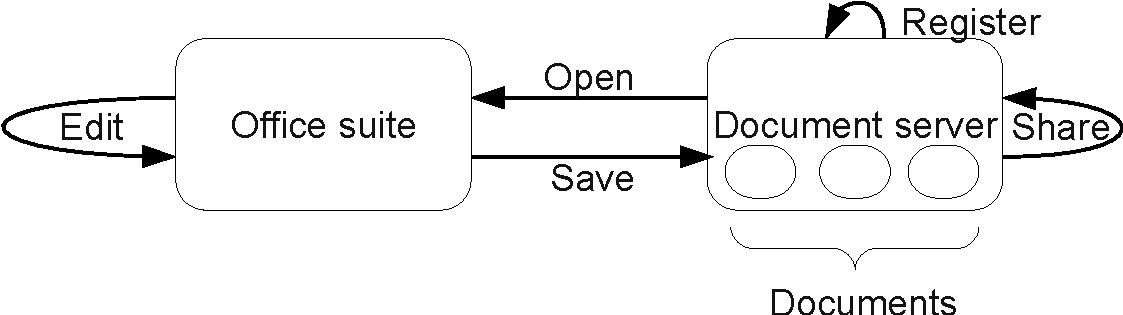
\includegraphics[width=300px,keepaspectratio]{general-arch-of-doc-mgmt-systems.pdf}
\caption{Architecture of a document management system}
\end{figure}

The document management server has registered users. Properties to users (full
name, email, password) are stored on the server.

Every user has document workspaces. Workspaces can have documents, links and
tasks. A workspace can be shared with different permissions (read-only,
read-write), and that is typically done by sending an invitation email which
the other user can accept.

A user may access the document server using a web browser, or via fat client
applications. The advantage of the web browser interface is that it can be
accessed from almost everywhere, however document editing can't be performed.
If such operation should be performed, then the user has to manually download
the document, edit then upload it. This method occasionally does not cause a
problem, but of course it's uncomfortable for daily work.

The other interface is a fat client, which is installed on the machine of the
user. Vendors like to produce a corresponding client for their server,
Microsoft Sharepoint and Microsoft Office is a typical setup.

It is important to note that of course a single server may serve multiple
clients. Also, the same client may connect to multiple servers, however in
practice a central server provides a document storage for all the collaborating
users.

In case of servers or clients speaking different communication protocols,
selection of the used protocol is selected differently on client and server
side. Servers can listen on different addresses, and in this case the address
identifies not only the server, but the used protocol as well.

For example Alfresco\cite{alfresco}, which is an open-source alternative to
Sharepoint, has its native protocol, but also (more or less) can speak the
Sharepoint protocol. As a result, it can be configured to listen on
\emph{http://project:8080/} as an Alfresco server, and on
\emph{http://localhost:7070} as a Sharepoint server.

Clients can have different extensions or plug-ins to handle different
protocols. For example Microsoft Office can accept Sharepoint URL-s in the
standard file opener dialog, while the Alfresco extension for OpenOffice.org
has a dedicated menu in the application to connect to an Alfresco server.

It is also common that the client extensions have minimal business logic. For
example the proprietary Sharepoint extension to OpenOffice.org, created by
Oracle can't talk to every Sharepoint server, like Microsoft Office does -- as
long as a server-side component provided by Oracle is not installed on the
server. While this approach may be compelling during development, actually it
is uncomfortable for system administrators.

As a result, I paid attention in my solution to not require such additional
server-side component installation.

\subsection{Related standards}
